
\begin{intro}
  \putindex{multigrid} Multigrid methods avoid the problems discussed
  in the section on two-level Schwarz methods by using not only two,
  but a whole hierarchy of mesh levels. On each level, an approximate
  solver, a so called smoother is employed, which improves the error
  somewhat, and then an approximation on a coarser level is used to
  improve further. This is done down to the coarsest level, where we
  assume that the solution process is cheap.
\end{intro}

\begin{Definition}{hierarchy-spaces}
  A \define{hierarchy of spaces} $\{V_\ell\}_0\le \ell \le L$ is a
  sequence of the form
  \begin{gather}
    V_0 \subset V_1 \subset \dots \subset V_L.
  \end{gather}
  We assume that $V_L = V$ is the high resolution space on which we
  want to solve~\eqref{eq:itintro:1}, but where the condition number
  of the matrix $\mat A$ is bad. On the other end of the spectrum, we
  assume that the solution of~\eqref{eq:itintro:1} on $V_0$ is easily
  possible.
\end{Definition}

\begin{Definition}{multigrid-method}
  A \define{multigrid method} consists of the following components:
  \begin{enumerate}
  \item A \define{smoother} $R_\ell$ acting on the level space
    $V_\ell$, usually an iterative method like Richardson, Jacobi,
    Gauss-Seidel or a Schwarz method.
  \item A \define{coarse grid solver} solving the problem on $V_0$
    exactly.
  \item Transfer operators between the levels $V_{\ell}$ and
    $V_{\ell+1}$. For standard finite element methods, this is
    typically the embedding operator. The transfer in opposite
    direction is achieved by the $L^2$-projection.
  \end{enumerate}
  
  On a given level $V_{\ell}$, the multigrid level consists of an
  alternating sequence of \putindex{smoothing step}s and
  \putindex{coarse grid correction}s, where the latter consist of a
  projection of the residual to the space $V_{\ell-1}$ and then
  recursive application of the same sequence. This is easiest
  described by the function
  \begin{subequations}
    \label{eq:mg:5}
  \begin{gather}
    \label{eq:mg:1}
    u_1 = MG_\ell(u^{(0)}, g),
  \end{gather}
  which takes an initial value $u^{(0)}$ and computes an approximation
  $u_1$ to the solution to $A_\ell u = g$ by the following scheme:
  first, for $\ell = 0$ let
  \begin{gather*}
    MG_0(u^{(0)}, g) = A_0^{-1} g_0.
  \end{gather*}
  On levels $\ell \neq 0$, perform the three steps
  \begin{itemize}
  \item Pre-smoothing: apply $m_{\text{pre}}$ steps of a Richardson
    iteration preconditioned with the smoother $R_\ell$:
    \begin{gather}
      \label{eq:mg:2}
      u^{(k+1)} = u^{(k)} - R_{\ell}^{-1} \left(A_\ell u^{(k)} - g_\ell\right),
      \qquad 0 \le k < m_{\text{pre}}.
    \end{gather}
    \item Coarse grid correction: let $v^{(0)} \in V_{\ell-1}$ and
      $g_{\ell-1} \in V_{\ell-1}^*$ such that
      \begin{gather}
        \label{eq:mg:3}
        g_{\ell-1} = \Pi_{\ell-1}^T \left(g_\ell - A_\ell u^{(m_{\text{pre}})}\right),
        \qquad
        v^{(0)} = 0.
      \end{gather}
      Then, compute 
      \begin{gather}
        \label{eq:mg:4}
        v^{(k+1)} = MG_{\ell-1}(v^{(k)}, g_{\ell-1}),
      \qquad 0 \le k < m_{\text{coarse}}.
      \end{gather}
      Let $w^{(0)} \in V_{\ell}$ be given by $w^{(0)} =
      u^{(m_{\text{pre}})} + v^{(m_{\text{coarse}})}$.
  \item Post-smoothing: apply $m_{\text{post}}$ steps of a Richardson
    iteration preconditioned with the smoother $R_\ell$:
    \begin{gather}
      \label{eq:mg:2a}
      w^{(k+1)} = w^{(k)} - R_{\ell}^{-1} \left(A_\ell w^{(k)} - g_\ell\right),
      \qquad 0 \le k < m_{\text{post}}.
    \end{gather}
    Assign $MG(u^{(0)}, g_\ell) = w^{(m_{\text{post}})}$.
  \end{itemize}    
  \end{subequations}
  
  This method has three parameters, the numbers of pre- and post
  smoothing steps $m_{\text{pre}}$ and $m_{\text{post}}$ as well as
  the number of coarse grid iterations $m_{\text{coarse}}$. Here, it
  is the last one which has a strong impact on the structure of the
  iteration. It defines what is called the \define{cycle type}, which
  is either \define{V-cycle} for $m_{\text{coarse}} = 1$ or
  \define{W-cycle} for $m_{\text{coarse}} = 2$. The structure of the
  cycles can be seen in Figure~\ref{fig:mg:1}.
\end{Definition}
\begin{figure}[tp]
  \centering
  \begin{minipage}[t]{.49\linewidth}
  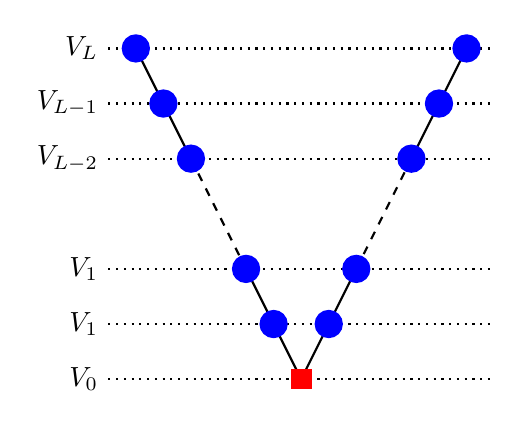
\begin{tikzpicture}[thick,scale=.7]
    % Levels
    \draw[dotted](0,0) node[anchor=east]{$V_0$} -- (7,0);
    \draw[dotted](0,1) node[anchor=east]{$V_1$} -- (7,1);
    \draw[dotted](0,2) node[anchor=east]{$V_1$} -- (7,2);
    \draw[dotted](0,4) node[anchor=east]{$V_{L-2}$} -- (7,4);
    \draw[dotted](0,5) node[anchor=east]{$V_{L-1}$} -- (7,5);
    \draw[dotted](0,6) node[anchor=east]{$V_L$} -- (7,6);
    
    % Transfers
    \draw(0.5,6) -- (1.5,4);
    \draw[dashed](1.5,4) -- (2.5,2);
    \draw(2.5,2) -- (3.5,0) -- (4.5,2);
    \draw[dashed](4.5,2) -- (5.5,4);
    \draw(5.5,4) -- (6.5,6);
    
    % Smoothers and coarse grid correction
    \node at (0.5,6) [circle,draw=blue,fill=blue] {};
    \node at (1.0,5) [circle,draw=blue,fill=blue] {};
    \node at (1.5,4) [circle,draw=blue,fill=blue] {};
    \node at (2.5,2) [circle,draw=blue,fill=blue] {};
    \node at (3.0,1) [circle,draw=blue,fill=blue] {};
    \node at (4.0,1) [circle,draw=blue,fill=blue] {};
    \node at (4.5,2) [circle,draw=blue,fill=blue] {};
    \node at (5.5,4) [circle,draw=blue,fill=blue] {};
    \node at (6.0,5) [circle,draw=blue,fill=blue] {};
    \node at (6.5,6) [circle,draw=blue,fill=blue] {};
    \node at (3.5,0) [rectangle,draw=red,fill=red] {};
  \end{tikzpicture}    
  \end{minipage}
  \begin{minipage}[t]{.49\linewidth}
  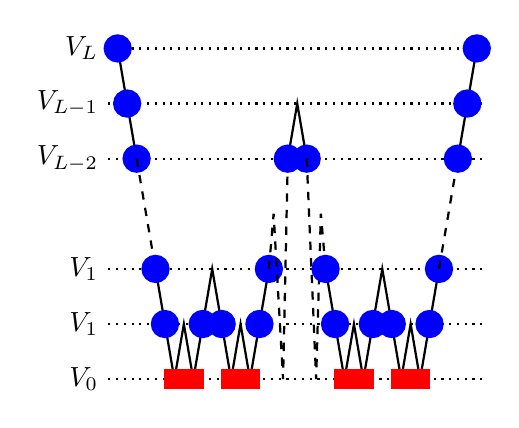
\begin{tikzpicture}[thick,yscale=.7,xscale=.6]
    % Levels
    \draw[dotted](0,0) node[anchor=east]{$V_0$} -- (8.0,0);
    \draw[dotted](0,1) node[anchor=east]{$V_1$} -- (8.0,1);
    \draw[dotted](0,2) node[anchor=east]{$V_1$} -- (8.0,2);
    \draw[dotted](0,4) node[anchor=east]{$V_{L-2}$} -- (8.0,4);
    \draw[dotted](0,5) node[anchor=east]{$V_{L-1}$} -- (8.0,5);
    \draw[dotted](0,6) node[anchor=east]{$V_L$} -- (8.0,6);

    % Transfers and smoothers
    \draw(0.2,6) node[circle,draw=blue,fill=blue] {}
    -- (0.4,5) node[circle,draw=blue,fill=blue] {}
    -- (0.6,4) node[circle,draw=blue,fill=blue] {};
    \draw[dashed](0.6,4) -- (1.0,2);
    \draw (1.0,2) node[circle,draw=blue,fill=blue] {}
    -- (1.2,1) node[circle,draw=blue,fill=blue] {}
    -- (1.4,0) node[rectangle,draw=red,fill=red] {}
    -- (1.6,1)
    -- (1.8,0) node[rectangle,draw=red,fill=red] {}
    -- (2.0,1) node[circle,draw=blue,fill=blue] {}
    -- (2.2,2)
    -- (2.4,1) node[circle,draw=blue,fill=blue] {}
    -- (2.6,0) node[rectangle,draw=red,fill=red] {}
    -- (2.8,1)
    -- (3.0,0) node[rectangle,draw=red,fill=red] {}
    -- (3.2,1) node[circle,draw=blue,fill=blue] {}
    -- (3.4,2) node[circle,draw=blue,fill=blue] {};
    \draw[dashed](3.4,2) -- (3.5,3) -- (3.7,0) -- (3.8,4);
    \draw(3.8,4) node[circle,draw=blue,fill=blue] {}
    -- (4.0,5)
    -- (4.2,4) node[circle,draw=blue,fill=blue] {};
    \draw[dashed] (4.2,4) -- (4.4,0) -- (4.5,3) 
    -- (4.6,2)
    ;
    \draw (4.6,2) node[circle,draw=blue,fill=blue] {}
    -- (4.8,1) node[circle,draw=blue,fill=blue] {}
    -- (5.0,0) node[rectangle,draw=red,fill=red] {}
    -- (5.2,1)
    -- (5.4,0) node[rectangle,draw=red,fill=red] {}
    -- (5.6,1) node[circle,draw=blue,fill=blue] {}
    -- (5.8,2)
    -- (6.0,1) node[circle,draw=blue,fill=blue] {}
    -- (6.2,0) node[rectangle,draw=red,fill=red] {}
    -- (6.4,1)
    -- (6.6,0) node[rectangle,draw=red,fill=red] {}
    -- (6.8,1) node[circle,draw=blue,fill=blue] {}
    -- (7.0,2) node[circle,draw=blue,fill=blue] {};
    \draw[dashed] (7.0,2) -- (7.4,4);
    \draw (7.4,4) node[circle,draw=blue,fill=blue] {}
    -- (7.6,5) node[circle,draw=blue,fill=blue] {}
    -- (7.8,6) node[circle,draw=blue,fill=blue] {};    
  \end{tikzpicture}    
  \end{minipage}
  \caption{Smoothing and grid transfer of the V-cycle (left) and
    W-cycle (right). Black lines indicate grid transfer, blue dots are
  smoothing operations and red squares are coarse grid
  solvers. ``Time'' is left to right.}
  \label{fig:mg:1}
\end{figure}

\begin{remark}
  Figure~\ref{fig:mg:1} shows that the recursive structure of the
  W-cycle is much more complex than that of the V-cycle. The
  complexity analysis below will show that higher values of
  $m_{\text{coarse}}$ do not lead to efficient algorithms.
\end{remark}

\begin{Definition}{variable-v-cycle}
  If the numbers of pre- and post smoothing steps in the V-cycle are
  dependent on the level $\ell$, we speak of the \define{variable
    V-cycle}. A typical choice is $m_\ell = 2^{L-\ell} m_L$, thus
  doubling the number of smoothing steps whenever stepping down one
  level.
\end{Definition}

\begin{note}
  The variable V-cycle with $m_\ell$ as mentioned in the previous
  definition has as many smoothing steps per iteration as the W-cycle.
\end{note}

\begin{remark}
  If we use an additive or multiplicative Schwarz method (omitting the
  coarse grid) as our smoother $R_\ell$, it should be possible in
  principle to use the analytical tools of
  Chapter~\ref{cha:iteration:schwarz-methods}. The difficulty then
  consists in ensuring that the spectral radius of the iteration
  matrix does not grow towards one if we proceed upwards on our scale
  of spaces $V_\ell$. This remark is a todo for the author and an
  encouragement for the reader. Hints may be found
  in~\cite{GriebelOswald95,Xu92}.
\end{remark}

\begin{remark}
  It turns out that the techniques used for the analysis of the
  V-cycle and the W-cycle, respectively are quite
  different. Therefore, we separate them into two sections.
\end{remark}

\begin{Theorem}{mg-complexity}
  Let $n_\ell$ be the dimension of $V_\ell$. Assume that the effort
  needed to for the operations in equations~\eqref{eq:mg:5}b/c/e is
  linear in $n_\ell$ and assume that $ n_{\ell+1}/n_\ell \approx 2^d$,
  where $d$ is the space dimension of the grid. Assume that the effort
  for the coarse grid solver is negligible. Then, the effort for
  one step of the V-cycle is of order $n_L$. The effort for one step
  of the W-cycle is of order $n_L$ for $d \ge 2$, while it is of order
  $n_L \log(n_L)$ in one dimension.
\end{Theorem}

\begin{proof}
  Start the recursion on level $L$ with the function $MG_L(0,
  g)$. This function calls $MG_{L-1}(\ldots)$ $m_{\text{coarse}}$
  times. Thus, by recursion, $MG_{\ell}(\ldots)$ is executed
  $m_{\text{coarse}}^{L-\ell}$ times.
  
  By our assumptions, the amount of operations $\breve N_\ell$ in $MG_\ell(\ldots)$
  without the coarse grid correction is linear in $n_\ell$, say
  bounded by $Cn_\ell$. Then, the overall effort $N_L$ on level $L$ is
  \begin{gather}
    \label{eq:mg:6}
    N_L \le C \sum_{\ell=1}^L n_\ell m_{\text{coarse}}^{L-\ell} \le C
    \sum_{\ell=1}^L n_L 2^{d(l-L)}m_{\text{coarse}}^{L-\ell}
    = C n_L \sum_{\ell=1}^L \left(\frac{m_{\text{coarse}}}{2^d}\right)^l.
  \end{gather}
  It remains to notice that the sum converges and is bounded
  independent of $L$ if and only if $m_{\text{coarse}}/2^d < 1$. The
  statements of the theorem follow immediately, observing that $L
  \simeq \log n_L$.
\end{proof}

\begin{Lemma}{mg-error-step}
  Let $B_\ell^{-1}$ be the operator associated with the action of the
  multigrid preconditioner on level $\ell$ for
  $\ell=0,\ldots,L$. Then, the error after one step of the multigrid
  method has the form
  \begin{gather}
    \label{eq:mg:7}
    u^{(k+1)} - u = E_L \left(u^{(k)} - u \right),
  \end{gather}
  where for $\ell=0,\ldots,L$ we denote by $E_\ell$ the
  \putindex{error propagation operator}
  \begin{gather}
    \label{eq:mg:8}
    E_\ell = \left(I-R_\ell^{-1} A_\ell\right)^{m_{\text{post}}}
    \left(I-B_{\ell-1}^{-1}A_{\ell-1} P_{\ell-1}\right)^{m_{\text{coarse}}}
     \left(I-R_\ell^{-1} A_\ell\right)^{m_{\text{pre}}}
  \end{gather}
\end{Lemma}

\begin{proof}
  For the smoother, we use the standard technique for Richardson's
  method outlined in Lemma~\ref{lemma:richardson:1}. For the coarse
  grid correction, we use Lemma~\ref{lemma:schwarz:2}.
\end{proof}

\begin{note}
  The structure of the error propagation operator~\eqref{eq:mg:8}
  already suggests the course of the multigrid analysis (as well as
  the design of smoothers). Namely, we will have to decompose $V_l$
  into $V_{l-1}$ and its $A$-orthogonal complement. Then, we use the
  induction argument that $I-B_{\ell-1}^{-1}A_{\ell-1}$ is is small on
  $V_{l-1}$, while bounded on its complement. Vice versa,
  $I-R_\ell^{-1} A_\ell$ must be bounded on all of $V_\ell$, while
  providing good reduction properties on the complement of $V_{l-1}$.
\end{note}

\section{The V-cycle}

\begin{assumption}
  \label{assumption:mg:1}
  Let the smoother $R_\ell$ be symmetric, positive definite and let
  the following two conditions hold, the second for some positive
  constant $\alpha$ independent of $\ell$:
  \begin{subequations}
    \label{eq:mg:9}
    \begin{xalignat}{2}
      \label{eq:mg:10}
      a\bigl((I-R_\ell^{-1}A_\ell)v,v\bigr) & \ge 0
      & \forall v &\in V_\ell, \\
      \label{eq:mg:20}
      r(w,w) &\le \alpha a(w,w)
      & \forall v &\in V_\ell, \quad w = (I-P_{\ell-1}) v
    \end{xalignat}
  \end{subequations}
\end{assumption}

\begin{Theorem}{v-cycle-convergence}
  Let $a(.,.)$ be symmetric, positive definite and let
  Assumption~\ref{assumption:mg:1} hold. Then, the V-cycle operator
  with $m_{\text{pre}} =m_{\text{post}} = m$ admits the estimate
  \begin{gather}
    \label{eq:mg:11}
    0 \le a(\bigl((I-B_\ell^{-1}A_\ell)v,v\bigr) \le \delta a(v,v),
    \qquad \forall v \in V_\ell,
  \end{gather}
  where
  \begin{gather}
    \label{eq:mg:12}
    \delta = \frac{\alpha}{\alpha+2m}.
  \end{gather}
  In particular, the contraction number of the multigrid method is
  bounded by a number less than 1, independent of the level.
\end{Theorem}

\begin{proof}
  \footnote{This version of the proof is taken
    from~\cite{ArnoldFalkWinther97Hdiv}. It can also be found
    in~\cite{BraessHackbusch83,Bramble93}.}
  First, abbreviate $K_{\ell} = I-R_{\ell}^{-1} A_\ell$, the error
  propagation operator of a smoothing step. Now we will prove the
  theorem by induction over $\ell$. First, since $B_0 = A_0$, it holds
  on level zero. For higher levels, we derive from~\eqref{eq:mg:8} the
  relation
  \begin{gather}
    \label{eq:mg:13}
    E_\ell = I-B_\ell^{-1} A_\ell = K_\ell^m\Bigl(
    (I-P_{\ell-1}) + (I-B_{\ell-1}^{-1} A_{\ell-1}) P_{\ell-1}
    \Bigr) K_\ell^m.
  \end{gather}
  Non-negativity follows readily by the induction argument and
  the same properties of the smoother and the Ritz-projection. For the
  upper bound, let $w = K_\ell^m v$ to obtain by the induction
  hypothesis
  \begin{multline}
    \label{eq:mg:14}
    a(E_\ell v,v) \le a\bigl((I-P_{\ell-1}) w,w\bigr) + \delta
    a(P_{\ell-1}w,w)
    \\
    = (1-\delta) a\bigl((I-P_{\ell-1}) w,w\bigr)
   + \delta a(w,w).
  \end{multline}
  Now we use the smoothing hypothesis anf the
  Bunyakovsky-Cauchy-Schwarz inequality for the bilinear form $r(.,.)$
  associated with the smoothing operator $R_\ell$ to obtain
  \begin{align*}
    a\bigl((I-P_{\ell-1}) w,w\bigr)
    &= \scal({(I-P_{\ell-1}) w}, A_\ell w) \\
    &= \scal(R_\ell {(I-P_{\ell-1})} w, R_\ell^{-1} A_\ell w)
    \\
    &= r\bigl((I-P_{\ell-1}) w, R_\ell^{-1} A_\ell w\bigr) \\
    &\le \sqrt{r\bigl((I-P_{\ell-1}) w,(I-P_{\ell-1}) w\bigr)}
    \sqrt{r\bigl(R_\ell^{-1} A_\ell w, R_\ell^{-1} A_\ell w\bigr)}
    \\
    &\le \sqrt{\alpha a\bigl((I-P_{\ell-1}) w,(I-P_{\ell-1}) w\bigr)}
    \sqrt{a\bigl(R_\ell^{-1} A_\ell w, w\bigr)}
  \end{align*}
  Using the projection property of $I-P_{\ell-1}$, we obtain
  \begin{gather}
    \label{eq:mg:15}
    a\bigl((I-P_{\ell-1}) w,w\bigr) \le \alpha a\bigl(R_\ell^{-1} A_\ell
    w, w\bigr)
    = \alpha a\bigl((I-K_\ell) K_\ell^{2m} v,v\bigr).
  \end{gather}
  
  The smoothing assumption also guarantees that the spectrum of
  $K_\ell$ is contained in the interval $[0,1]$. Therefore,
  \begin{gather}
    \label{eq:mg:16}
    a\bigl((I-K_\ell) K_\ell^{2m} v,v\bigr)
    \le a\bigl((I-K_\ell) K_\ell^{i} v,v\bigr),
    \qquad i=0,\dots,2m,
  \end{gather}
  yielding by deflating the telescoping sum
  \begin{gather}
    \label{eq:mg:17}
    a\bigl((I-K_\ell) K_\ell^{2m} v,v\bigr)
    \le \frac1{2m} \sum_{i=0}^{2m-1}
    a\bigl((I-K_\ell) K_\ell^{i} v,v\bigr)
    = \frac1{2m} a\bigl((I-K_\ell^{2m}) v,v\bigr)
  \end{gather}
  Combining~\eqref{eq:mg:14}, \eqref{eq:mg:15}, and~\eqref{eq:mg:17},
  we obtain
  \begin{gather}
    \begin{split}
      a(E_\ell v,v) &\le (1-\delta)\frac\alpha{2m}
      a\bigl((I-K_\ell^{2m}) v,v\bigr)
      + \delta a(K_\ell^m v,K_\ell^m v)
      \\
      &= (1-\delta)\frac\alpha{2m} a(v,v)
      + \left(\delta - (1-\delta)\frac\alpha{2m}\right)
      a(K_\ell^m v,K_\ell^m v).
    \end{split}
  \end{gather}
  Finally, we enter $\delta=\alpha/(\alpha+2m)$ to obtain
  \begin{gather*}
    \delta - (1-\delta)\frac\alpha{2m} = 0,
  \end{gather*}
  and thus
  \begin{gather}
    \label{eq:mg:18}
    a(E_\ell v,v) \le \left(1-\frac\alpha{\alpha+2m}\right)\frac\alpha{2m}
    a(v,v) = \frac\alpha{\alpha+2m}a(v,v). 
  \end{gather}
\end{proof}

\begin{Lemma}{mg-additive}
  Let $R_\ell$ be the scaled additive Schwarz method
  \begin{gather}
    \label{eq:mg:19}
    R_a^{-1} = \omega \sum_{j=1}^J P_j A^{-1},
  \end{gather}
  where the subspaces $V_j$ are defined by overlapping subdomains
  $\Omega_j$ as in~\eqref{eq:schwarz:9}. Not that we do not include
  the coarse space here. Then, for $\omega$ sufficiently small, this
  smoother fulfills Assumption~\ref{assumption:mg:1}.
\end{Lemma}

\begin{proof}
  The positive definiteness and symmetry of the smoother have been
  proven in an abstract way in Lemma~\ref{lemma:schwarz:3}. In order
  to prove estimate~\eqref{eq:mg:10}, we observe that by
  Lemma~\ref{lemma:schwarz:5} and Lemma~\ref{lemma:schwarz:6}
  \begin{gather*}
    r(v,v) = \omega \min_{v=\sum v_j} a(v_j, v_j) \gtrsim \omega a(v,v),
  \end{gather*}
  where the implicit constant depends on the number of overlaps in
  Definition~\ref{definition:schwarz:finite-covering}. Thus, we can
  choose $\omega$ independent of $\ell$ such that
  \begin{gather*}
    r(v,v) \ge a(v,v) \qquad \forall v\in V_\ell.
  \end{gather*}
  Accordingly, $R_\ell - A_\ell$ is positive definite, and since
  $R_\ell^{-1}$ is as well, so is $I-R_\ell^{-1} A_\ell$.
  It remains to prove~\eqref{eq:mg:20}, but this is exactly the second
  half of the proof of Lemma~\ref{lemma:schwarz:stable-decomposition},
  if we replace the Clément interpolant into the coarse space by the
  Ritz projection.
\end{proof}

%\section{The W-cycle and two-grid convergence}


%%% Local Variables: 
%%% mode: latex
%%% TeX-master: "main"
%%% End: 
